\documentclass[letterpaper,11pt]{article}
\usepackage{xeCJK}
\usepackage{bm}
\usepackage{geometry}
\usepackage{amssymb}
\usepackage{amsmath}
\usepackage[cal=boondoxo, scr=dutchcal]{mathalfa}
\usepackage{multirow}
\usepackage[unicode, CJKbookmarks=true]{hyperref}

\numberwithin{equation}{section}

\geometry{a4paper,left=2cm,right=2cm,top=2cm,bottom=2cm}

\usepackage{setspace}
\setstretch{1.1}
\setlength{\parskip}{0.1\baselineskip}

\usepackage{graphicx}
\usepackage{caption}

\usepackage[backend=biber, style=ieee]{biblatex}
\addbibresource{ref.bib}

% 可选:设置URL显示样式
\urlstyle{APACsame} % 使URL使用正文字体
\def\UrlFont{\rmfamily} % 使用罗马字体而非等宽字体

\begin{document}

\title{AI分享}
\author{张驰}
\maketitle

\begin{figure}[htbp]
    \centering
    
\includegraphics[width=1\textwidth]{../../assets/imgs/ai_share/bg.jpg}
    \caption*{黑客帝国动画版(2003)海报}
\end{figure}

\section{引子}

近年,AI对不少行业都形成了一定的冲击,大家对AI的热情也愈发高涨。
写这篇文章的目的是希望以简单直观的方式介绍大模型领域的常见概念,比如各种时髦的名词与新兴技术(像是AI Agent、Function Call、MCP等)。
帮助大家了解当前的热点技术与工具,当工作中涉及AI时,可以有一定的判断。
这篇文章主要讲解大模型相关技术与工具的背景、功能与使用场景,对于这些背后的原理只做简单阐述,如果有兴趣可以进一步阅读参考链接。

\section{大模型的工作原理}

在阐述大模型相关的技术与工具前,需要大家首先对大模型的工作原理有一定了解。
对于大模型的详细工作原理可参阅文献\cite{alammar2018transformer}。
其实大模型的工作原理很简单,就是四个字“文字接龙”,大模型根据输入的 Prompt 计算出下一个可能的字或词,再用此 Prompt 附加上新产生的字或词作为大模型新的输入,重复此过程直至得到完整的结果,大模型的简易工作原理如图所示。

\begin{figure}[htbp]
    \centering
    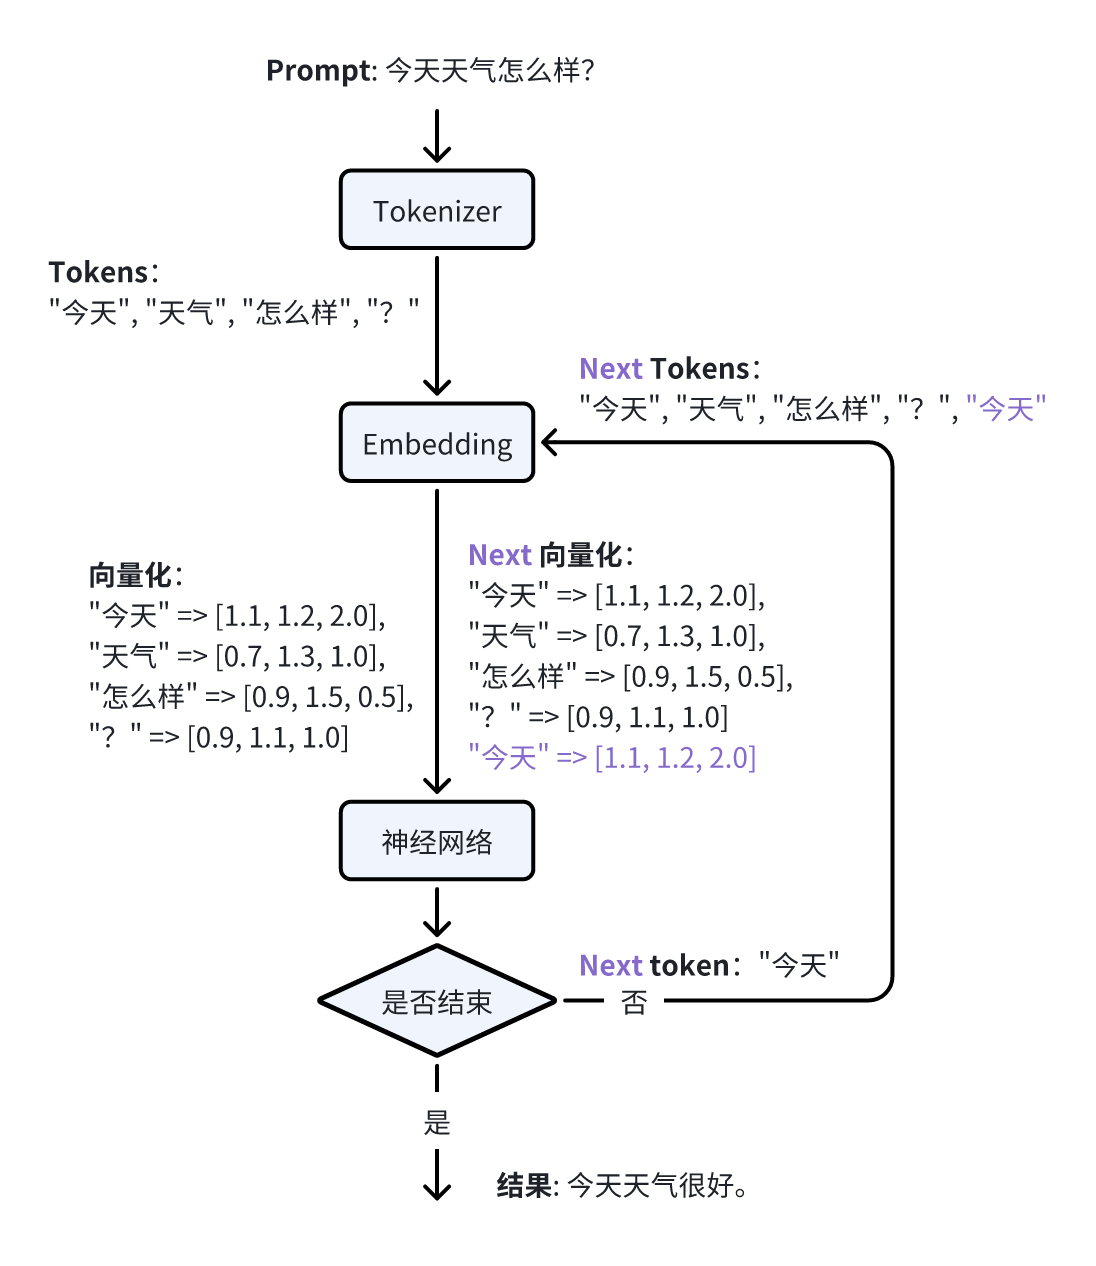
\includegraphics[width=0.7\textwidth]{../../assets/imgs/ai_share/llm_workflow.png}
    \caption{大模型的工作流程}
    \label{llm-workflow}
\end{figure}

\printbibliography[title={引用}]

\end{document}